\section{Paging: Introduction}

%------------------------------------------------
\begin{frame}{Two Approaches to Space Management}

\begin{itemize}
    \item \textbf{Variable-sized pieces} (e.g., segmentation):
          space becomes \textbf{fragmented} and allocation gets harder over time.
    \item \textbf{Fixed-sized pieces}: the idea of \textbf{paging},
          going back to the Atlas system.
    \item The address space is divided into fixed-sized units called \textbf{pages}.
    \item Physical memory is viewed as an array of fixed-sized slots called
          \textbf{page frames}; each frame holds a single virtual page.
\end{itemize}

\begin{block}{The Crux: How to Virtualize Memory with Pages}
How can we virtualize memory with pages, so as to avoid the problems of
segmentation? How do we make it work well, with minimal space and time
overheads?
\end{block}

\end{frame}

%------------------------------------------------
\begin{frame}{A Simple Example}

\begin{itemize}
    \item Tiny address space: 64 bytes, four 16-byte pages (VP 0--3).
    \item Physical memory: 128 bytes, eight page frames; virtual pages are placed
          at different locations, and the OS uses some frames for itself.
    \item Real address spaces are much bigger (32 or 64 bits).
\end{itemize}

\begin{columns}[c]
    \begin{column}{0.42\textwidth}
        \begin{figure}
        \centering
        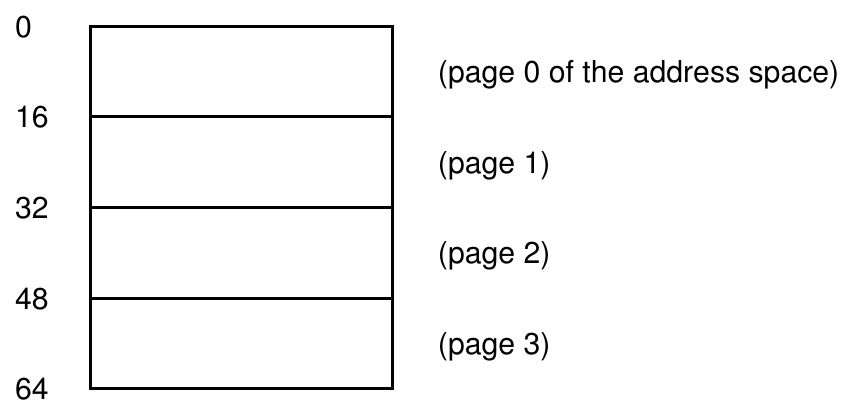
\includegraphics[height=0.25\textheight]{figs/chapter-18/figure-18.1.png}
        \caption*{Source: chapter page 2.}
        \label{fig:figure-18.1}
        \end{figure}
    \end{column}
    \begin{column}{0.52\textwidth}
        \begin{figure}
        \centering
        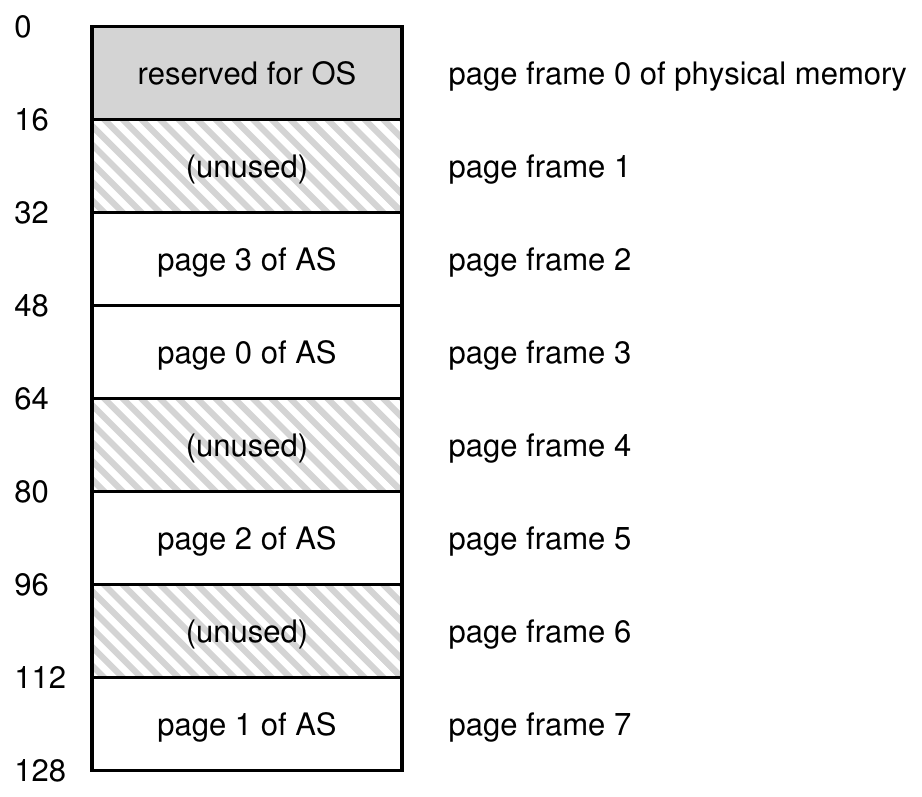
\includegraphics[height=0.42\textheight]{figs/chapter-18/figure-18.2.png}
        \caption*{Source: chapter page 2.}
        \label{fig:figure-18.2}
        \end{figure}
    \end{column}
\end{columns}

\end{frame}

%------------------------------------------------
\begin{frame}{Advantages of Paging}

\begin{itemize}
    \item \textbf{Flexibility}: supports the address-space abstraction
          regardless of how a process uses it
          (no assumptions about heap and stack growth direction).
    \item \textbf{Simple free-space management}:
    \begin{itemize}
        \item to place a 4-page address space, the OS just finds four free frames;
        \item e.g., by taking the first four entries of a free list of frames.
    \end{itemize}
    \item In the example: VP~0~$\rightarrow$~PF~3, VP~1~$\rightarrow$~PF~7,
          VP~2~$\rightarrow$~PF~5, VP~3~$\rightarrow$~PF~2;
          frames 1, 4 and 6 are free.
\end{itemize}

\end{frame}

%------------------------------------------------
\begin{frame}{The Page Table}

\begin{itemize}
    \item A \textbf{per-process} data structure that stores
          \textbf{address translations} for each virtual page.
    \item It tells where in physical memory each page resides.
    \item Another process has its own page table, since its virtual pages
          map to different physical frames (modulo sharing).
    \item Exception discussed later: the \textbf{inverted page table}.
\end{itemize}

\begin{block}{Aside: Data Structure --- The Page Table}
One of the most important data structures of the memory-management subsystem.
Its structure is determined by the hardware (older systems) or managed more
flexibly by the OS (modern systems).
\end{block}

\end{frame}

%------------------------------------------------
\begin{frame}{Splitting the Virtual Address}

\begin{itemize}
    \item A virtual address is split into:
    \begin{itemize}
        \item \textbf{virtual page number (VPN)};
        \item \textbf{offset} within the page.
    \end{itemize}
    \item 64-byte address space $\Rightarrow$ 6-bit addresses ($2^6 = 64$).
    \item 16-byte pages $\Rightarrow$ 4-bit offset; 4 pages $\Rightarrow$ 2-bit VPN.
\end{itemize}

\begin{center}
\renewcommand{\arraystretch}{1.3}
\begin{tabular}{|c|c|c|c|c|c|}
\multicolumn{2}{c}{VPN} & \multicolumn{4}{c}{offset} \\
\hline
Va5 & Va4 & Va3 & Va2 & Va1 & Va0 \\
\hline
\end{tabular}
\end{center}

\end{frame}

%------------------------------------------------
\begin{frame}[fragile]{Address Translation Example}

\begin{columns}[T]

\column{0.50\textwidth}
\begin{itemize}
    \item \texttt{movl 21, \%eax}
    \item $21 = 010101_2$: VPN $= 01$ (page 1), offset $= 0101$ (byte 5).
    \item Page table: VP~1~$\rightarrow$ \textbf{PFN} 7 ($111_2$).
    \item Replace the VPN with the PFN; the \textbf{offset is not translated}.
    \item Physical address: $1110101_2 = 117$.
    \item PFN is also called physical page number (PPN).
\end{itemize}

\column{0.45\textwidth}
\begin{figure}
    \centering
    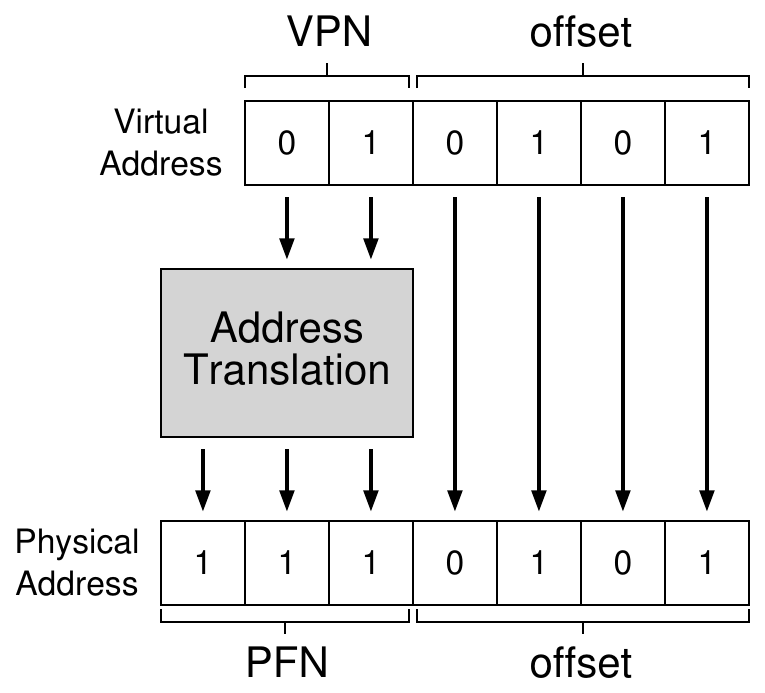
\includegraphics[width=1.0\linewidth]{figs/chapter-18/figure-18.3.png}
    \caption*{Source: chapter page 4.}
    \label{fig:figure-18.3}
\end{figure}

\end{columns}

\end{frame}

%------------------------------------------------
\begin{frame}{Where Are Page Tables Stored?}

\begin{columns}[T]

\column{0.55\textwidth}
\begin{itemize}
    \item Page tables can get \textbf{terribly large}.
    \item 32-bit address space, 4KB pages:
          20-bit VPN + 12-bit offset.
    \item $2^{20}$ translations ($\approx$ 1 million) per process.
    \item 4 bytes per \textbf{page table entry (PTE)}
          $\Rightarrow$ \textbf{4MB} per page table.
    \item 100 processes $\Rightarrow$ 400MB just for translations!
    \item Hence, page tables are not kept in on-chip MMU hardware,
          but \textbf{in memory} (for now, OS physical memory).
\end{itemize}

\column{0.40\textwidth}
\begin{figure}
    \centering
    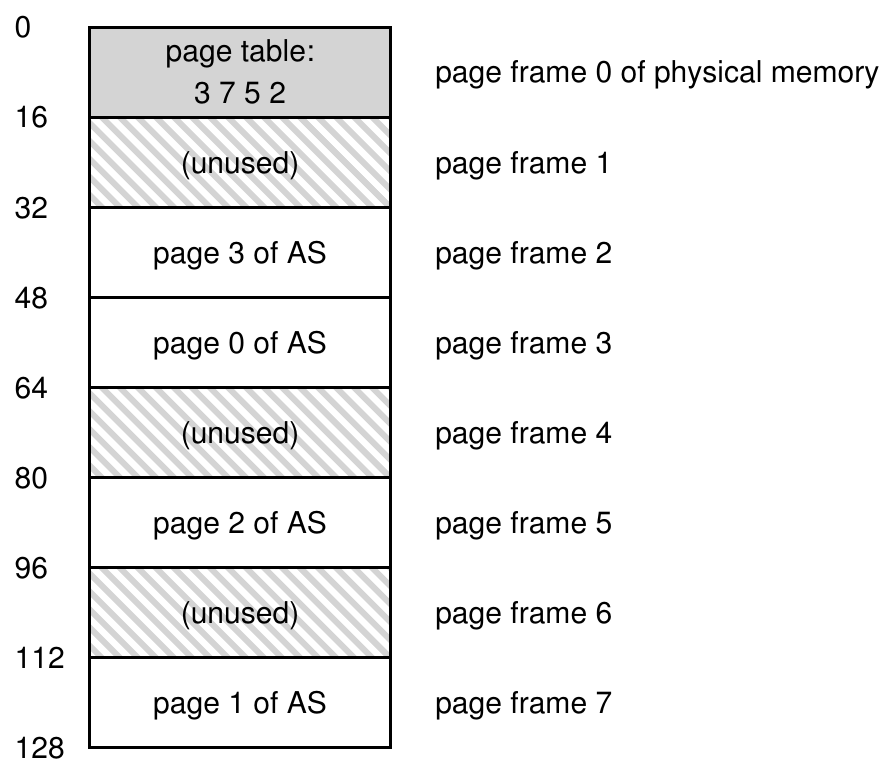
\includegraphics[width=1.0\linewidth]{figs/chapter-18/figure-18.4.png}
    \caption*{Source: chapter page 5.}
    \label{fig:figure-18.4}
\end{figure}

\end{columns}

\end{frame}

%------------------------------------------------
\begin{frame}{What's Actually in the Page Table?}

\begin{itemize}
    \item Any data structure could map VPNs to PFNs.
    \item Simplest form: \textbf{linear page table} --- an array indexed by VPN,
          whose entry (PTE) holds the PFN.
    \item Common PTE bits:
    \begin{description}
        \item[Valid] whether the translation is valid; unused space is marked
              invalid (trap on access). Crucial for \textbf{sparse} address spaces.
        \item[Protection] whether the page can be read, written, or executed.
        \item[Present] whether the page is in memory or on disk (swapped out).
        \item[Dirty] whether the page was modified since brought into memory.
        \item[Reference] (accessed) whether the page has been accessed;
              useful for page replacement.
    \end{description}
\end{itemize}

\end{frame}

%------------------------------------------------
\begin{frame}{Example: An x86 Page Table Entry}

\begin{figure}
    \centering
    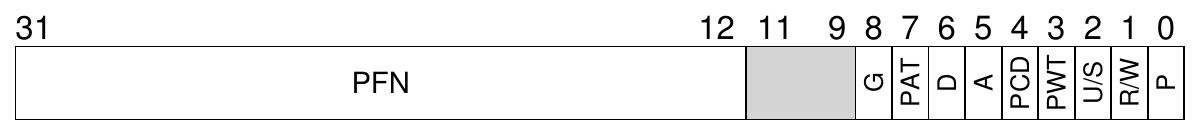
\includegraphics[width=0.9\linewidth]{figs/chapter-18/figure-18.5.png}
    \caption*{Source: chapter page 7.}
    \label{fig:figure-18.5}
\end{figure}

\begin{itemize}
    \item \textbf{P}: present; \textbf{R/W}: writes allowed;
          \textbf{U/S}: user-mode access allowed.
    \item \textbf{PWT, PCD, PAT, G}: hardware caching behavior.
    \item \textbf{A}: accessed; \textbf{D}: dirty; and the \textbf{PFN} itself.
    \item No separate valid bit: if $P=0$, the OS uses its own structures to
          decide whether the page is valid (swap it in) or not (illegal access).
\end{itemize}

\end{frame}

%------------------------------------------------
\begin{frame}[fragile]{Paging: Also Too Slow}

\begin{itemize}
    \item A \textbf{page-table base register} holds the physical address of
          the page table of the running process.
    \item To locate the PTE:
\end{itemize}

\begin{block}{Finding the PTE}
\small
\texttt{VPN = (VirtualAddress \& VPN\_MASK) >> SHIFT}\\
\texttt{PTEAddr = PageTableBaseRegister + (VPN * sizeof(PTE))}
\end{block}

\begin{itemize}
    \item In the example: \texttt{VPN\_MASK} $=$ \texttt{0x30} ($110000_2$),
          \texttt{SHIFT} $=4$.
    \item Then fetch the PTE, extract the PFN, and concatenate with the offset:
\end{itemize}

\begin{block}{Forming the Physical Address}
\small
\texttt{offset = VirtualAddress \& OFFSET\_MASK}\\
\texttt{PhysAddr = (PFN << SHIFT) | offset}
\end{block}

\end{frame}

%------------------------------------------------
\begin{frame}[fragile]{Accessing Memory with Paging}

\begin{lstlisting}[style=CStyle]
// Extract the VPN from the virtual address
VPN = (VirtualAddress & VPN_MASK) >> SHIFT
// Form the address of the page-table entry (PTE)
PTEAddr = PTBR + (VPN * sizeof(PTE))
// Fetch the PTE
PTE = AccessMemory(PTEAddr)
// Check if process can access the page
if (PTE.Valid == False)
    RaiseException(SEGMENTATION_FAULT)
else if (CanAccess(PTE.ProtectBits) == False)
    RaiseException(PROTECTION_FAULT)
else
    // Access OK: form physical address and fetch it
    offset   = VirtualAddress & OFFSET_MASK
    PhysAddr = (PTE.PFN << PFN_SHIFT) | offset
    Register = AccessMemory(PhysAddr)
\end{lstlisting}

\end{frame}

%------------------------------------------------
\begin{frame}{Two Real Problems}

\begin{itemize}
    \item Every memory reference (instruction fetch, load or store) requires
          \textbf{one extra memory reference} to fetch the translation.
    \item This will likely slow down the process by a factor of two or more.
\end{itemize}

\begin{alertblock}{Without careful hardware and software design, page tables\ldots}
\begin{itemize}
    \item cause the system to run \textbf{too slowly};
    \item take up \textbf{too much memory}.
\end{itemize}
\end{alertblock}

\end{frame}

%------------------------------------------------
\begin{frame}[fragile]{A Memory Trace: Setup}

\begin{columns}[T]

\column{0.48\textwidth}
\begin{lstlisting}[style=CStyle]
int array[1000];
...
for (i = 0; i < 1000; i++)
    array[i] = 0;
\end{lstlisting}

{\footnotesize
\begin{verbatim}
1024 movl $0x0,(%edi,%eax,4)
1028 incl %eax
1032 cmpl $0x03e8,%eax
1036 jne  1024
\end{verbatim}
}

\column{0.48\textwidth}
\begin{itemize}
    \item 64KB address space, 1KB pages.
    \item Linear page table at physical address 1KB (1024).
    \item Code: VPN~1~$\rightarrow$~PFN~4.
    \item Array (VA 40000--44000):
          VPN~39--42 $\rightarrow$ PFN~7--10.
\end{itemize}

\end{columns}

\end{frame}

%------------------------------------------------
\begin{frame}{A Memory Trace: Results}

\begin{columns}[T]

\column{0.45\textwidth}
\begin{itemize}
    \item Each instruction fetch: one page-table access + the fetch.
    \item The \texttt{mov} adds a page-table access + the array access.
    \item \textbf{10 memory accesses per iteration}:
    \begin{itemize}
        \item 4 instruction fetches;
        \item 1 explicit memory update;
        \item 5 page-table accesses.
    \end{itemize}
\end{itemize}

\column{0.52\textwidth}
\begin{figure}
    \centering
    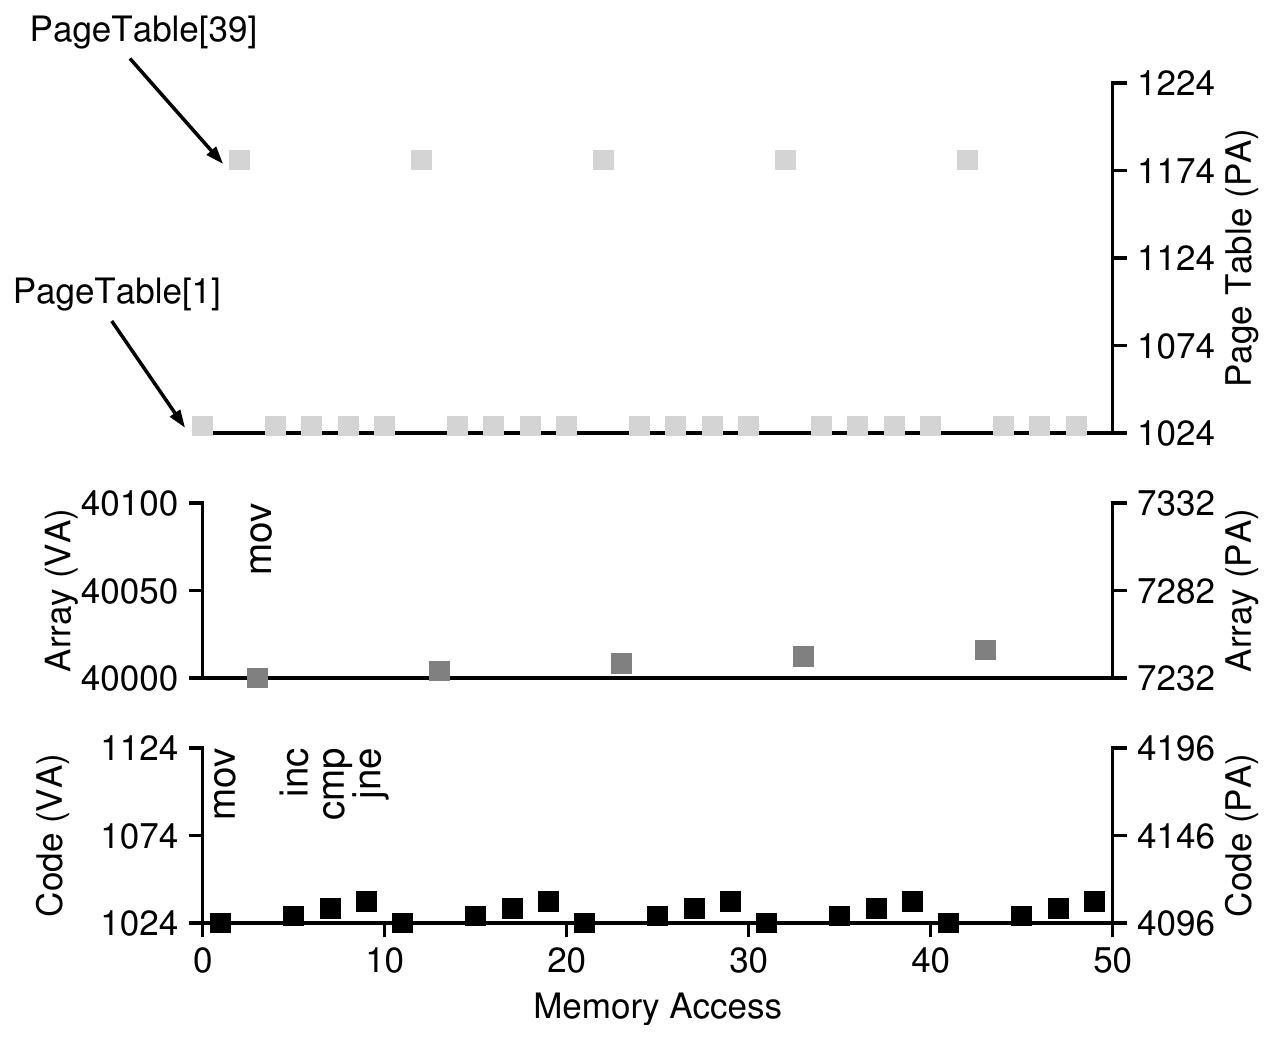
\includegraphics[width=0.9\linewidth]{figs/chapter-18/figure-18.7.png}
    \caption*{Source: chapter page 11.}
    \label{fig:figure-18.7}
\end{figure}

\end{columns}

\begin{block}{Question}
What changes as the loop runs beyond the first five iterations?
\end{block}

\end{frame}

%------------------------------------------------
\begin{frame}{Summary}

\begin{itemize}
    \item \textbf{Paging} divides memory into fixed-sized units.
    \item Advantages over segmentation:
    \begin{itemize}
        \item no \textbf{external fragmentation};
        \item flexibility, enabling \textbf{sparse} use of address spaces.
    \end{itemize}
    \item A naive implementation leads to:
    \begin{itemize}
        \item a \textbf{slower machine} (extra memory accesses to the page table);
        \item \textbf{memory waste} (memory filled with page tables).
    \end{itemize}
    \item The next chapters show how to make paging work well.
\end{itemize}

\end{frame}

%------------------------------------------------
\begin{frame}{Homework (Simulation)}

\begin{itemize}
    \item Simulator: \texttt{paging-linear-translate.py}.
    \item How does linear page table size change as:
    \begin{itemize}
        \item the address space grows?
        \item the page size grows? Why not use big pages in general?
    \end{itemize}
    \item What happens as the percentage of allocated pages (\texttt{-u})
          increases?
    \item Which parameter combinations are unrealistic? Why?
    \item What happens if the address space is bigger than physical memory?
\end{itemize}

\end{frame}
